%% The '3p' and 'times' class options of elsarticle are used for Elsevier CRC
%% The 'procedia' option causes ecrc to approximate to the Word template
\documentclass[3p,times,procedia]{elsarticle}
\flushbottom

%% The `ecrc' package must be called to make the CRC functionality available
\usepackage{ecrc}
\usepackage[colorlinks=true]{hyperref}%url}
\usepackage{amsmath}
\usepackage{epstopdf}
\usepackage{todonotes}
\usepackage{color}

\newcommand{\andrey}[1]{\textcolor{blue}{#1}}
\newcommand{\emanuel}[1]{\textbf{\color{CarnationPink}#1}}

\newcommand{\egtodo}[2]{\todo[inline,backgroundcolor=orange!20!white]{\textcolor{cyan}{{\bf \it by: #1}:  {\bf Emanuel:} #2}}}
\newcommand{\jltodo}[2]{\todo[inline,backgroundcolor=orange!20!white]{\color{Maroon}{{\bf \it by: #1}: {\bf James:} #2}}}
\newcommand{\aatodo}[2]{\todo[inline,backgroundcolor=orange!20!white]{\color{red}{{\bf \it by: #1}: {\bf Andrey:}  {\huge BLERG!!!!}: #2}}}

%% The ecrc package defines commands needed for running heads and logos.
%% For running heads, you can set the journal name, the volume, the starting page and the authors

%% set the volume if you know. Otherwise `00'
\volume{00}

%% set the starting page if not 1
\firstpage{1}

%% Give the name of the journal
\journalname{Physics Procedia}

%% Give the author list to appear in the running head
%% Example \runauth{C.V. Radhakrishnan et al.}
\runauth{A. E. Antipov et al.}

%% The choice of journal logo is determined by the \jid and \jnltitlelogo commands.
%% A user-supplied logo with the name <\jid>logo.pdf will be inserted if present.
%% e.g. if \jid{yspmi} the system will look for a file yspmilogo.pdf
%% Otherwise the content of \jnltitlelogo will be set between horizontal lines as a default logo

%% Give the abbreviation of the Journal.
\jid{phpro}

%% Give a short journal name for the dummy logo (if needed)
\jnltitlelogo{Physics Procedia}


\usepackage{amssymb}
%% The amsthm package provides extended theorem environments
%% \usepackage{amsthm}

%% The lineno packages adds line numbers. Start line numbering with
%% \begin{linenumbers}, end it with \end{linenumbers}. Or switch it on
%% for the whole article with \linenumbers after \end{frontmatter}.
%% \usepackage{lineno}

%% natbib.sty is loaded by default. However, natbib options can be
%% provided with \biboptions{...} command. Following options are
%% valid:

%%   round  -  round parentheses are used (default)
%%   square -  square brackets are used   [option]
%%   curly  -  curly braces are used      {option}
%%   angle  -  angle brackets are used    <option>
%%   semicolon  -  multiple citations separated by semi-colon
%%   colon  - same as semicolon, an earlier confusion
%%   comma  -  separated by comma
%%   numbers-  selects numerical citations
%%   super  -  numerical citations as superscripts
%%   sort   -  sorts multiple citations according to order in ref. list
%%   sort&compress   -  like sort, but also compresses numerical citations
%%   compress - compresses without sorting
%%
\biboptions{authoryear}

% \biboptions{}

% if you have landscape tables
\usepackage[figuresright]{rotating}
%\usepackage{harvard}
% put your own definitions here:x
%   \newcommand{\cZ}{\cal{Z}}
%   \newtheorem{def}{Definition}[section]
%   ...

% add words to TeX's hyphenation exception list
%\hyphenation{author another created financial paper re-commend-ed Post-Script}

% declarations for front matter

\begin{document}

\begin{frontmatter}

%% Title, authors and addresses

%% use the tnoteref command within \title for footnotes;
%% use the tnotetext command for the associated footnote;
%% use the fnref command within \author or \address for footnotes;
%% use the fntext command for the associated footnote;
%% use the corref command within \author for corresponding author footnotes;
%% use the cortext command for the associated footnote;
%% use the ead command for the email address,
%% and the form \ead[url] for the home page:
%%
%% \title{Title\tnoteref{label1}}
%% \tnotetext[label1]{}
%% \author{Name\corref{cor1}\fnref{label2}}
%% \ead{email address}
%% \ead[url]{home page}
%% \fntext[label2]{}
%% \cortext[cor1]{}
%% \address{Address\fnref{label3}}
%% \fntext[label3]{}

\dochead{28th Annual CSP Workshop on ``Recent Developments in Computer Simulation Studies in Condensed Matter Physics'', CSP 2015}
%% Use \dochead if there is an article header, e.g. \dochead{Short communication}
%% \dochead can also be used to include a conference title, if directed by the editors
%% e.g. \dochead{17th International Conference on Dynamical Processes in Excited States of Solids}

\title{opendf - an implementation of the dual fermion method for strongly correlated systems }

%% use optional labels to link authors explicitly to addresses:
%% \author[label1,label2]{<author name>}
%% \address[label1]{<address>}
%% \address[label2]{<address>}



\author[a]{Andrey E. Antipov\corref{cor1}} 
\author[a]{James P.F. LeBlanc}
\author[a]{Emanuel Gull}

\address[a]{Department of Physics, University of Michigan, Ann Arbor, Michigan 48109, USA}

\begin{abstract}
We present the \textbf{opendf} code, an open-source implementation of the dual fermion method : a multiscale approach for solving lattice problems of interacting strongly correlated systems. Our code as provided is applicable to Hubbard models in dimensions $D=1,2,3,4$. The method is built on the dynamical mean field theory as a starting point and hence utilizes the DMFT input: Green's function and full vertex functions. As an output, the code provides an estimate for spatially dependent static and dynamic susceptibilities and Green's functions. The code is distributed as an open-source package under MIT license. 
\end{abstract}

\begin{keyword}
Type your keywords here, separated by semicolons ; 

%% keywords here, in the form: keyword \sep keyword

%% PACS codes here, in the form: \PACS code \sep code

%% MSC codes here, in the form: \MSC code \sep code
%% or \MSC[2008] code \sep code (2000 is the default)

\end{keyword}
\cortext[cor1]{Corresponding author.}
\end{frontmatter}

%\correspondingauthor[*]{Corresponding author. Tel.: +0-000-000-0000 ; fax: +0-000-000-0000.}
\email{aantipov@umich.edu}

%%
%% Start line numbering here if you want
%%
% \linenumbers

%% main text

%\enlargethispage{-7mm}
\vspace*{-8pt}

\listoftodos
\aatodo{}{Insert references if you can.}

\section{Introduction}

Providing solutions to interacting problems which extend beyond analytically tractible mean-field approaches is a long standing avenue of modern physics research.  Great strides in this problem were made in the advent of the numerically tractable procedure of dynamical mean-field theory (DMFT), capable of providing time and frequency dependent information.  A very general theory, DMFT is applicable to any Hamiltonian which can be separated into local and non-local contributions.  DMFT then provides an approximate solution by solving the local correlations exactly.

It is now the case for standard strong interacting systems, such as the D-dimensional Hubbard model, that solutions of DMFT are available from existing software simulation packages such as ALPS (Algorithms and Libraries for Physics Simulations), ALPSCore (the core elements of ALPS), TRIQS (Toolbox for Research on Interacting Quantum Systems:  applications of LDA + DMFT).\egtodo{}{Need to discuss if refering to Alpscore makes sense.  Does not have prebuilt DMFT application?}

With this in mind, we present opendf, a code which performs the Dual Fermion self consistency within a ladder approximation to build non-local correlations on top of the solutions provided by existing DMFT routines.  The implementation here is intended to be general, and not model specific.  By taking input of the local Green's function and full vertex function from DMFT, opendf produces an output of momentum and frequency dependent self energies and green's functions, as well as the $Q$ scattering vector dependence of two-particle susceptibilities.  While the treatment here is approximate [only a subset of higher order diagrams are considered] the results of DF are a robust improvement over the DMFT approximation.  We will see that computational complexity of this additional step above DMFT is not substantial and give two example applications using analytic results in the atomic limit as well as input from DMFT for the Hubbard model in two-dimensions.


\section{Methodology}
\subsection{Prerequisites}
Consider the Hamiltonian, $H$, for a lattice fermionic model in $D$ dimensions,
\begin{equation}
H = \sum_{k\sigma} (\varepsilon_k - \mu) c^\dagger_{k\sigma} c_{k\sigma} + \sum_i H^{\mathrm{int}} [c^\dagger_i, c_i],
\end{equation}
written in mixed momentum, $k$, and realspace, $i$, notation in terms of creation and annihilation operators ($c^\dagger_{k\sigma}$ and $c_{k\sigma}$ respectively).  The index $\sigma$ labels the spin projection, $\varepsilon_k$ is the lattice dispersion relation and $k$ is the vector in the reciprocal space. 
$H^{\mathrm{int}}$ is the local interaction for each site, $i$, on the lattice. 
No assumption is made within DF as to the structure of $H^{\mathrm{int}}$.  For example, $H^{\mathrm{int}} = U c^\dagger_\uparrow c_\uparrow c^\dagger_\downarrow c_\downarrow$ would refer to the typical Hubbard model [Hubbard1963]. 

As a first step, which must be performed outside of this code, an approximate solution of the model is obtained from a dynamical mean field calculation. \egtodo{}{Can we pick a good DMFT reference here. ALPS? Or something else?}
It provides an estimate for the local Green's function of the lattice problem as a  solution of the Anderson impurity model, embedded into a self-consistently determined hybridization. The imaginary time action of this ``impurity problem''  reads  
\begin{equation}
S^{\mathrm{A}} = -\sum_{i\omega,\sigma} (i\omega + \mu - \Delta_{\omega\sigma}) c^*_{\omega\sigma} c_{\omega\sigma} + S^{\mathrm{int}},
\end{equation}
where $S^{int} = \int_0^\beta d\tau H^{\mathrm{int}} [c^\dagger_i(\tau), c_i(\tau)] $ is the interaction part of the action and $\Delta_{\omega\sigma}$ is a self-consistently determined hybridization function []. 
The one particle Green's function $g_{\omega\sigma} = -\langle c_{\omega\sigma} c^\dagger_{\omega\sigma} \rangle$ of the of the Anderson impurity model and the two particle vertex functions (i.e. the connected parts of two-particle Green's functions)  
\begin{equation}\label{eqn:vertex}
\gamma_{\Omega\omega\omega'}^{\sigma_1\sigma_2\sigma_3\sigma_4} = \left(\langle c_{\omega,\sigma_1} c^\dagger_{\Omega + \omega,\sigma_2} c_{\omega' + \Omega, \sigma_3} c^\dagger_{\omega', \sigma_4}\rangle - g_{\omega\sigma_1}g_{\omega'\sigma_3}\delta_{\Omega,0}\delta_{\sigma_1,\sigma_2} + g_{\omega\sigma_1} g_{\omega + \Omega, \sigma_2} \delta_{\omega,\omega'}\delta_{\sigma, \sigma_3} \right)
\end{equation}
are the input to DF calculations. 

The presented version of the code considers spin-symmetric solutions of the lattice $s=1/2$ fermionic problems, and does not describe symmetry-broken phases. We will omit the spin index $\sigma$ in single particle quantities in what follows, such that the complete set of input quantities reads
\begin{itemize}
\item $g_\omega$ - the full Green's function of the DMFT impurity problem (same values for both spin components)
\item $\Delta_{\omega}$ - hybridization function of the DMFT impurity problem
\item $\mu$ - chemical potential of the problem
\item Two independent components of the impurity vertex function, $\gamma_{\Omega\omega\omega'}^{\sigma_1\sigma_2\sigma_3\sigma_4}$, from Eqn~\eqref{eqn:vertex}: $\gamma_{\Omega,\omega,\omega'}^{\uparrow\uparrow\uparrow\uparrow} \equiv \gamma^{\uparrow\uparrow}_{\Omega,\omega,\omega'} $ and $\gamma_{\Omega,\omega,\omega'}^{\uparrow\downarrow\downarrow\uparrow} \equiv  \gamma^{\uparrow\downarrow}_{\Omega,\omega,\omega'} $
%\item Lattice dispersion $\varepsilon_{k}$ and the dimensionality $D$ are compiled into the specific running executable. The hypercubic lattice dispersion $-2t \sum_{i=1}^d \cos k_i$ at dimensions $D=1,2,3,4$ is provided with the code. Other lattice choices can be achieved by extending the code. 
\end{itemize}

\subsection{Ladder dual fermion self-consistency loop}
A precise derivation of the DF equations can be found in [], here we outline the equations solved with the code. The evaluation of the DF equations consists of iterative updates of the fully dressed dual fermion Green's function $\tilde G$, until convergence is achieved. It starts with the construction of the bare dual fermion propagator
\begin{equation}
\tilde G^{(0)}_{\omega,k} = \left[g_{\omega}^{-1} + \Delta_\omega - \varepsilon_k\right]^{-1} - g_{\omega}, \label{eq:gd0}
\end{equation}
which represents a $k$-dependent correction to the impurity Green's function. This Green's function is used to construct bubbles: 
\begin{equation}\label{eq:dual_bubble}
\tilde \chi_{\Omega\omega}(q) = -\frac{T}{N_k^d} \sum_k \tilde G_{\omega, k} \tilde G_{\omega + \Omega, k+q}.
\end{equation}
Here the integral over the Brilloin zone is replaced with a discrete summation with $N_k$ points in each direction. The impurity vertex functions are combined into density and magnetic channels (labeled d/m respectively) as: 
\begin{equation}\label{eq:spin_symm}
\gamma^{d/m}_{\Omega,\omega,\omega'} = \gamma^{\uparrow\uparrow}_{\Omega,\omega,\omega'} \pm \gamma^{\uparrow\downarrow}_{\Omega,\omega,\omega'}
\end{equation}
The vertices for the respected channels from Eq. \ref{eq:spin_symm} and the bubbles from Eq. \ref{eq:dual_bubble} are substituted into ladder equations:
\begin{equation}\label{eq:dual_ladder}
\Gamma^{d/m}_{\Omega,\omega,\omega'}(q) = \gamma^{d/m}_{\Omega,\omega,\omega'} + \sum_{\omega''} \gamma^{d/m}_{\Omega,\omega,\omega''} \tilde\chi_{\Omega,\omega''}(q) \Gamma^{d/m}_{\Omega'',\omega'}(q).
\end{equation}

Evaluation of Eq. \ref{eq:dual_ladder} is performed independently for each pair of vertex bosonic frequency $\Omega$ and transferred momentum $q$. 
$\gamma_{\Omega,\omega,\omega'}$ and $\Gamma_{\Omega,\omega,\omega'}(q)$ are represented as matrices in the space of fermionic Matsubara frequencies $\omega$, $\omega'$, and $\tilde\chi_{\Omega,\omega''}(q)$ is a diagonal matrix. 
In the matrix notation for each $\Omega$ and $q$ this equation reads 
\begin{equation}\label{eq:lin_alg_inv}
(\hat 1 - \hat \gamma \tilde \chi)\hat \Gamma  = \hat \gamma.
\end{equation} 
This equation is physically correct only when the maximum eigenvalue of $\hat \gamma \tilde \chi$ is smaller than one, i.e. all eigenvalues of the matrix $\hat D = \hat 1 - \hat \gamma \tilde \chi$ are positive. 
To determine it, an LU-decomposition of the matrix $\hat D$ is performed, and a determinant $D(\Omega, q)$ is calculated.
If $D(\Omega, q) > 0$, then Eq. \ref{eq:lin_alg_inv} is solved and $\Gamma$ is obtained at constant computational complexity.
When $D(\Omega, q) \leq 0$, the DF solution is outside of the convergence radius of the ladder approximation.
Given that the resulting solution is unique, one can extend this convergence radius by doing a low-order iterative evaluation of $\Gamma$ and checking if the inversion of Eq. \ref{eq:dual_ladder} can be obtained on the next DF iteration. 
 
Once the fully dressed vertex function $\Gamma_{\Omega,\omega,\omega'}$ is obtained, it is used in the Schwinger-Dyson equation to obtain the fermionic self-energy $\tilde \Sigma_{\omega, k}$. 
The equation reads:
\begin{equation}\label{eq:sd}
\tilde \Sigma_{\omega, k} = \frac{T}{2 N_k^d}  \sum_{\Omega, q} \left( 3 \left[\Gamma^m_{\Omega,\omega,\omega}(q) - \frac{1}{2}\Gamma^{(2), m}_{\Omega,\omega,\omega}(q) \right] + \Gamma^d_{\Omega,\omega,\omega}(q) - \frac{1}{2}\Gamma^{(2), d}_{\Omega,\omega,\omega}(q)  \right) \tilde G_{\omega, k + q},
\end{equation}
where $\Gamma^{(2)} = \hat \gamma \tilde \chi \hat \gamma $ indicates the second order (first iteration) correction from Eq. \ref{eq:dual_ladder} to avoid diagrammatic overcounting. 

The resulting self-energy is used to feed back the dual Green's function through the Dyson's equation:
\begin{equation}\label{eq:dyson}
\tilde G^{-1}_{\omega k} = \left[G^{(0}_{\omega k}\right]^{-1} - \tilde \Sigma_{\omega k}
\end{equation}

The procedure is repeated until convergence of $\tilde G$ is achieved. 

\subsection{Resulting observables}
Once the fully converged dual Green's function $\tilde G$, and consequently, self-energy $\tilde \Sigma$, vertices $\Gamma^{d/m}$ are obtained, they can be used in determining the lattice correlators. Specifically, 
\begin{itemize}
\item Lattice self-energy: 
\begin{equation}\label{eq:sigma_lat}
\Sigma_{\omega, k} = \frac{\tilde \Sigma_{\omega, k}}{1 - g_\omega \Sigma_{\omega, k}} + \Sigma^{DMFT}_{\omega},
\end{equation}
where $\Sigma^{DMFT}_{\omega} = i\omega + \mu - \Delta_{\omega} - g_\omega^{-1}$. 
\item Lattice Green's function
\begin{equation}\label{eq:glat}
G_{\omega,k} = \left[\Delta_{\omega} - \varepsilon_{k}\right]^{-1} + \left[\Delta_{\omega} - \varepsilon_{k}\right]^{-1} g_{\omega}^{-1} \tilde G_{\omega, k} g_{\omega}^{-1} \left[\Delta_{\omega} - \varepsilon_{k}\right]^{-1}.
\end{equation}
Eqs. \ref{eq:sigma_lat} and \ref{eq:glat} are related through a Dyson's equation for $G$ and $\Sigma$. 
\item Charge/Spin susceptibility 
\begin{align}
\chi^{\mathrm{ch/sp}} (\Omega, q) & = -T \sum_{\omega k} G_{\omega k} G_{\omega+\Omega k+q} + \sum_{\omega,\omega'} L_{\Omega, \omega}(q) \Gamma^{d/m}_{\Omega,\omega,\omega'}(q) L_{\Omega, \omega'}(q), \\
L_{\Omega, \omega}(q) & = -T \sum_k \mathfrak{G}_{\omega,k} \mathfrak{G}_{\omega + \Omega,k + q} \\
\mathfrak{G}_{\omega,k} & = \tilde G_{\omega k} \frac{\tilde G^{(0)}_{\omega, k} + g_\omega}{\tilde G^{(0)}_{\omega, k}}
\end{align}
\end{itemize}

\section{Distribution and Implementation}
The code is distributed as a C++ library with compiled executables \texttt{hub\_df\_cubic{\bf D}d}, where \texttt{\bf D} labels the number of dimensions ($D=1,2,3,4$). We use the opensource \texttt{gftools} library \cite{gftools} for algebraic operations with single- and multi-particle Green's functions and it's interface to the \texttt{ALPSCore} libraries \cite{ALPSCore} for loading/saving \texttt{hdf5} objects. Calculation of bubbles of Green's functions is performed using FFT transformations. The loop through the Brilloin zone in Eq. \ref{eq:sd} is optimized by sampling only the irreducible wedge and reweighting contributions from different symmetry points. The code is available on \url{https://github.com/aeantipov/opendf}.

The library distribution allows for flexibility with the input data. In order to use provided \texttt{hub\_df\_cubic{\bf D}d} executables the input data should be stored in the \texttt{hdf5} file, under any chosen group name. It should contain the following objects, loadable by \texttt{gftools} routines. 
\begin{itemize}
\item \texttt{/gw0} and \texttt{/gw1}. $g_{\omega \uparrow}$ and $g_{\omega \downarrow}$.  Assumed to be identical.
\item \texttt{/delta0} and \texttt{/delta1}, storing $\Delta_\omega$.
\item \texttt{/F00} and \texttt{/F01}. $\gamma^{\uparrow\uparrow}$ and $\gamma^{\uparrow\downarrow}$ respectively.
\item Other parameters, like $\mu$ and hopping unit are provided through the provided command line interface.
\end{itemize}
The example input generator for the case of $U \gg t$ (the case of  ``atomic limit'') and particle-hole symmetric regime is provided with the code, in which 
\begin{align}\label{eq:atomic_limit1}
g_{\omega} & = \frac{1}{2}\left[\frac{1}{i\omega - U/2} + \frac{1}{i\omega + U/2}\right] \\
\Delta_{\omega} & = 2Dg_{\omega} \label{eq:atomic_limit2} \\ 
\gamma^{\uparrow\uparrow}_{\Omega,\omega,\omega'} & = \frac{\beta U^2}{4} (\delta_{\omega_1,\omega_2} - \delta_{\omega_1,\omega_4} ) \Lambda_{\omega_1}\Lambda_{\omega_3} \label{eq:atomic_limit3} \\ 
\label{eq:atomic_limit4}
\gamma^{\uparrow\downarrow}_{\Omega,\omega,\omega'} & = -U + 
\frac{U^3}{8}\frac{\omega_1^2 + \omega_2^2 + \omega_3^2 + \omega_4^2}{\omega_1^2\omega_2^2\omega_3^2\omega_4^2} + \frac{3U^5}{16}\frac{1}{\omega_1\omega_2\omega_3\omega_4}  \\
& \notag + \frac{\beta U^2}{4} \frac{1}{1 + \exp(\beta U /2 )} 
(2\delta_{ \omega_2, -\omega_3} + \delta_{\omega_1, \omega_2}) 
\Lambda_{\omega_2} \Lambda_{\omega_3}  \\ 
& \notag - \frac{\beta U^2}{4} \frac{1}{1 + \exp(-\beta U /2 )} 
(2\delta_{ \omega_1, \omega_4} + \delta_{\omega_1, \omega_2}) 
\Lambda_{\omega_1} \Lambda_{\omega_3},
\end{align}
where $\Lambda_\omega = 1 + U^2/(4\omega^2)$ and fermionic notation $\omega_1 = \omega, \omega_2 = \omega + \Omega, \omega_3 = \omega' + \Omega, \omega_4 = \omega'$ are used to simplify the notation.

The output of the code is stored in a generated or existing hdf5 file under the \texttt{/df} section.

\section{Performance}

The numerical solution of dual fermion equations requires introducing several control parameters. In particular,
the vertex function $\gamma_{\Omega,\omega,\omega'}$ is sampled on a grid with a cutoff $N_\Omega$ in bosonic and $N_{\omega}$ fermionic frequencies and the Brilloin zone is sampled on a finite grid of size $N_k$, providing the total volume of the system $N=N_k^d$. We analyze the convergence of the code upon tuning $N_{\Omega}$, $N_{\omega}$ and $N_k$ and the computational scaling below. Eqs. \ref{eq:atomic_limit1}, \ref{eq:atomic_limit2}, \ref{eq:atomic_limit3}, \ref{eq:atomic_limit4} are used to provide the input to the code and the system is evaluated in $2$ dimensions, at $U=8$, $\mu = \frac{U}{2}$. We choose the value of $g= \tilde G_{i\pi / \beta, 0, 0}$ to control the convergence. After making several runs, changing control parameter $N_x$, with $x = \{ \Omega, \omega, k \}$, we extrapolate the value to $N_x \to \infty$ and plot the normalized difference 
\begin{align}\label{eqn:deltag}
\delta_{g} = \left|\frac{g_{N_x} - g_{N_x \to \infty}}{g_{N_x \to \infty}}\right|
\end{align}
to evaluate the error. The maximum run-time of this benchmark data is $\approx 4$ min.

\begin{figure}[ht]
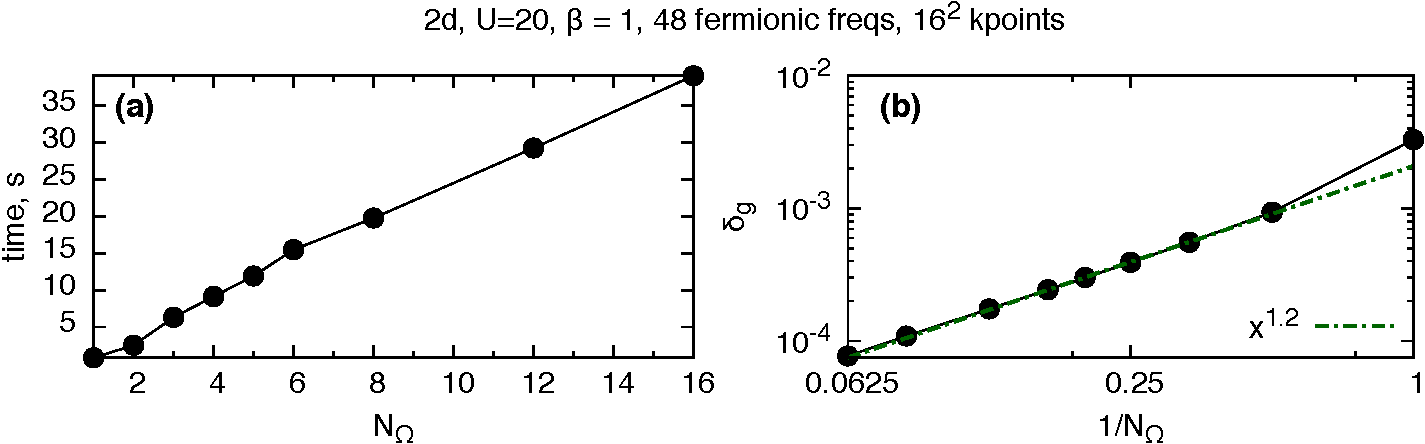
\includegraphics[width=1.0\columnwidth]{time_bfreqs.pdf}
\caption{(a) Execution time as a function of the number of bosonic frequencies $N_{\Omega}$; (b) Systematic error $\delta_g$ of the dual fermion Green's function $\tilde G_{i\omega, k}$ at $i\omega = i\pi / \beta, k = (0,0)$ for the Hubbard model in 2 dimensions at different number of bosonic frequencies $N_b$. (c) $\delta_g(N_{\Omega})$ in a logarithmic scale. }
\label{fig:benchmark_b}
\end{figure}

Fig. \ref{fig:benchmark_b} shows the performance of the \texttt{opendf} code upon the change of the total number of bosonic frequencies in the vertex $\gamma_{\Omega}$ for a fixed number of fermionic frequencies $N_{\omega}=48$ for a $16 \times 16$ k-space grid. The computational effort, indicated by the time to convergence in Fig.~\ref{fig:benchmark_b}(a), grows linearly in $N_{\Omega}$, while the error, as defined in Eqn.~\ref{eqn:deltag} and shown in frame (b), is on the order of a few percent and decreases quadratically, indicating that this error can be eliminated with large enough $N_{\Omega}$.

\begin{figure}[ht]
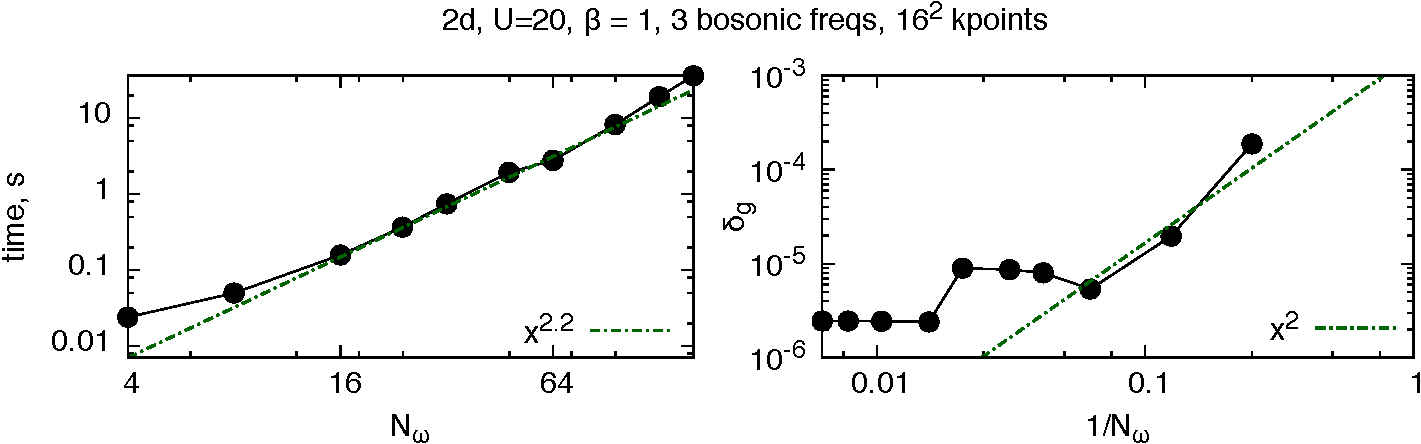
\includegraphics[width=1.0\columnwidth]{time_ffreqs.pdf}
\caption{(a) Execution time (log scale in (b); (c) Systematic error $\delta_g$ as a function of the number of used fermionic frequencies $N_{\omega}$. (d) is the zoom of $\delta_g(N_{\omega}$ dependence at large $N_{\omega}$.}
\label{fig:benchmark_f}
\end{figure}

We analyze the performance of the code with respect to the change of the total number of fermionic frequencies in Fig. \ref{fig:benchmark_f}.  In this benchmark we fix the number of bosonic frequencies, $N_{\Omega}=4$, and perform the calculation on a $16\times16$ k-space grid. The computational scaling seen in Fig.~\ref{fig:benchmark_f}(a)  grows quadratically, while the relative error shown in Fig.~\ref{fig:benchmark_f}(b) remains an order of magnitude smaller, as compared to the variation in $N_{\Omega}$ shown in Fig.\ref{fig:benchmark_b}(b). We see that $g$ converges very quickly with an increase of $N_{\omega}$ and for large values of $N_{\omega}$ the scaling stops and becomes constant.

\begin{figure}[ht]
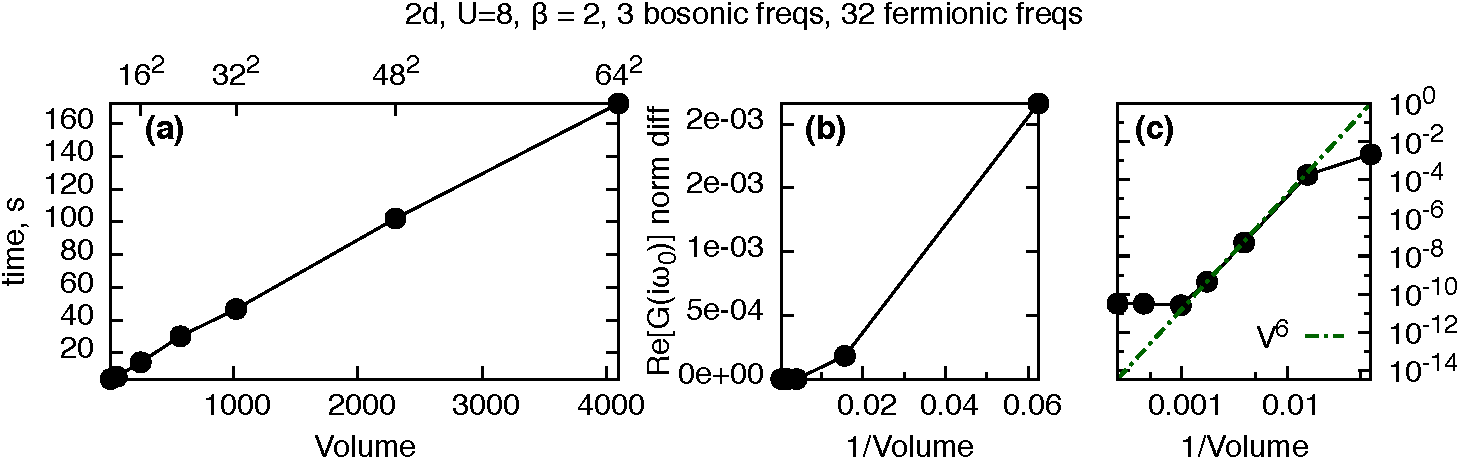
\includegraphics[width=1.0\columnwidth]{time_kpts.pdf}
\caption{(a) Execution time as a function of Volume=$N_k^d$. (b) Systematic error $\delta_g$ as a function of the volume. (c) log-scale of (b).}
\label{fig:benchmark_kpts}
\end{figure}

The performance of the code with respect to the change of number of k-space samples within the Brilloin zone, is plotted on Fig. \ref{fig:benchmark_kpts}. The computational effort (frame (a)) scales linearly with the volume $N_k^d$ of the system and the error is very small and scales as $(N_k^d)^6$, until it reaches the floating point precision.

\section{Examples}

\aatodo{}{Atomic limit example please.  }

Next we illustrate an example of output from opendf using input from single particle Green's functions and two-particle vertex functions obtained using a DMFT code built upon the ALPS libraries.[cite alps here I guess]  The results for the real part of the self energy are shown in Fig.~\ref{fig:hub_atomic} for $U/t=8$ and $U/t=12$. The DMFT gives a zero contribution to this part of the self energy due to particle-hole symmetry in this case.  However, using this result as input to opendf produces a strongly momentum dependent self energy.  

\begin{figure}[ht]
\centering
\includegraphics[width=0.6\columnwidth]{DF_U12.eps}
\caption{Dual Fermion result for the momentum dependence of the real part of the self energy at momenta $(k_x, k_y)$ throughout the Brillouin zone, for the 2D Hubbard model at half-filling, at $\beta=2$, and for interaction strengths $U/t=8$ and $12$.}
\label{fig:hub_atomic}
\end{figure}


\section{Conclusion}
In these proceedings we have introduced the opendf project which contains command line tools to solve the dual fermion self consistency conditions and computes non-local corrections to the local solutions provided by DMFT.  As such, opendf fills an important void in the existing available software packages, allowing for quick implementations of the DF technique on top of existing DMFT routines.  

The code, which is available at \url{https://github.com/aeantipov/opendf} will continue to undergo development.  Goals include incorporating ... \aatodo{}{What are some future directions with the code?} ex. annealing/extending radius of convergence.... different choices of sampled diagrams, attempt at determining accuracy by checking the contributions of higher order diagrams, 


\section*{Acknowledgements}
Authors are grateful to D. Hirschmeier for fruitful discussions and acknowledge the Simons collaboration on the many-electron problem for financial support and for it's support of the \texttt{ALPSCore} project.

\end{document}


